% !Mode:: "TeX:UTF-8" 

 

\BiSection{3.17}{Figures}

\fancyhead[R]{本题3.17由QC.Z完成}

解:

\scalebox{3}{(a)}

当$V_{in}<V_{TH1}$时$M_1$关,而$M_2$导通于是$V_{out}=0$,$M_2$在深线性区

之后当$V_{in}>V_{TH1}$时$M_1$进入饱和区,$M_2$进入线性区。然后在达到临界条件$V_{out}=V_{b}-V_{TH2}$时$M_2$进入饱和区

最后$V_{in}=V_{DD}$时$V_{out}=V_{DD}-V_{GS1}$

		\begin{figure}[H] %H为当前位置,!htb为忽略美学标准,htbp为浮动图形
	\begin{minipage}{\linewidth}
		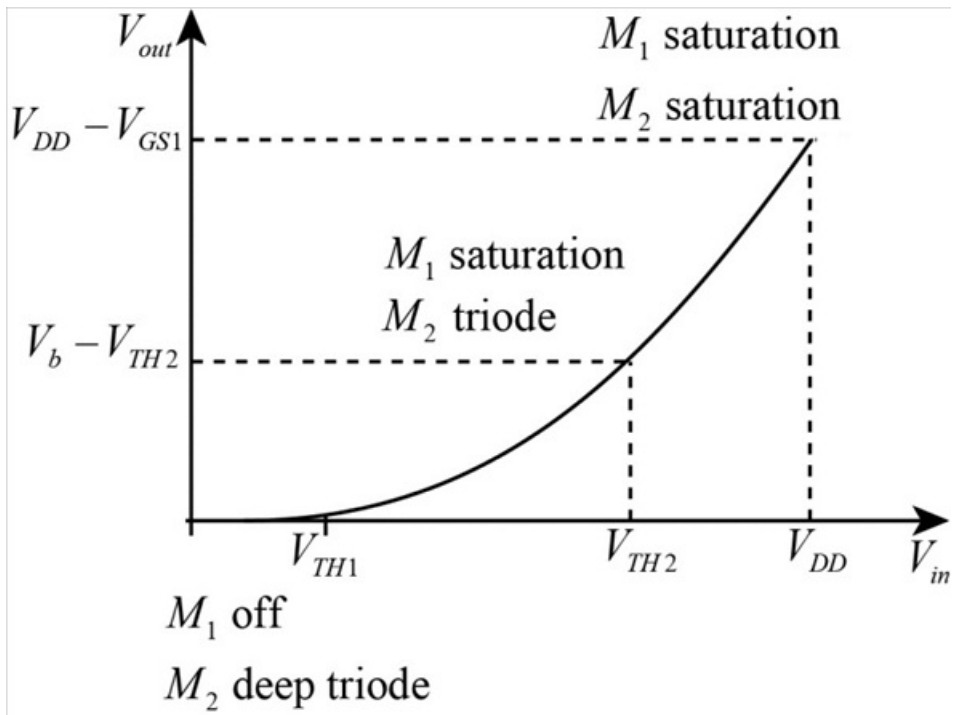
\includegraphics[width=1\linewidth]{3.17-1}
	\end{minipage}
	\caption*{图1} %最终文档中希望显示的图片标题
\end{figure}

\color{green}{
	
	\{
	
	横轴的$V_{TH2}=V_{b}-V_{TH2}+V_{GS1}$
	
	\}
	
}

\color{black}{}

\scalebox{3}{(b)}

当$V_{in}<V_{TH1}$时$M_1,M_2$关,而$M_3$导通于是$V_{out}=V_{DD}$,$M_3$在深线性区

之后当$V_{in}>V_{TH1}$时,又因为$M_1,M_2$的漏源电压高所以$M_1,M_2$进入饱和区。$M_1$栅源电压增大后漏电流增大,$M_3$为满足电流导致$V_{out}$下降。$M_3$进入线性区。

然后在达到临界条件$V_{out}=V_{b2}-V_{TH3}$时$M_3$进入饱和区


然后在达到临界条件$V_{in}-V_{TH1}=V_{b1}-V_{GS2}$,即$V_{in}=V_{b1}-V_{GS2}+V_{TH1}$时$M_1$进入线性区

		\begin{figure}[H] %H为当前位置,!htb为忽略美学标准,htbp为浮动图形
	\begin{minipage}{\linewidth}
		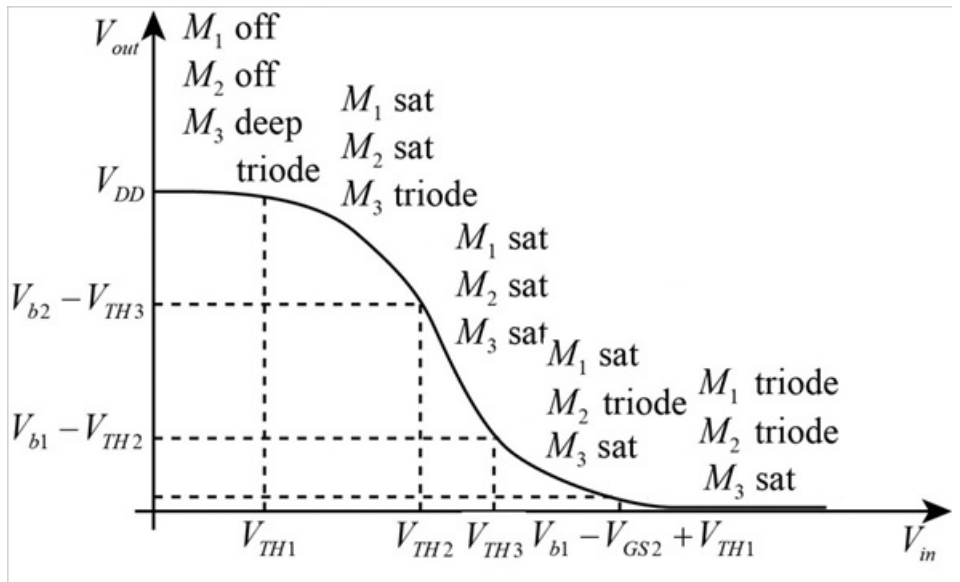
\includegraphics[width=1\linewidth]{3.17-2}
	\end{minipage}
	\caption*{图2} %最终文档中希望显示的图片标题
\end{figure}

\scalebox{3}{(c)}

$M_3$关时$V_{out}=V_{DD}$

然后输入电压增加,$M_3$进入线性区

然后在临界条件$V_{out}=V_{in}-V_{TH3}$被满足时$M_3$进入饱和区

然后在临界条件$V_{out}=V_{b1}-V_{TH2}$被满足时$M_2$进入线性区

然后在达到临界条件$V_{out}-V_{DS2}=V_{b2}-V_{TH1}$,即$V_{out}=V_{b2}-V_{TH1}+V_{DS2}$时$M_1$进入线性区

当$V_{in}=V_{DD}-V_{TH3}$时$M_3$关,$V_{out}=0$,$M_1,M_2$在深线性区

%当$V_{in}=V_{DD}-V_{TH3}$时$M_3$关,而$M_1,M_2$导通于是$V_{out}=0$,$M_1,M_2$在深线性区

		\begin{figure}[H] %H为当前位置,!htb为忽略美学标准,htbp为浮动图形
	\begin{minipage}{\linewidth}
		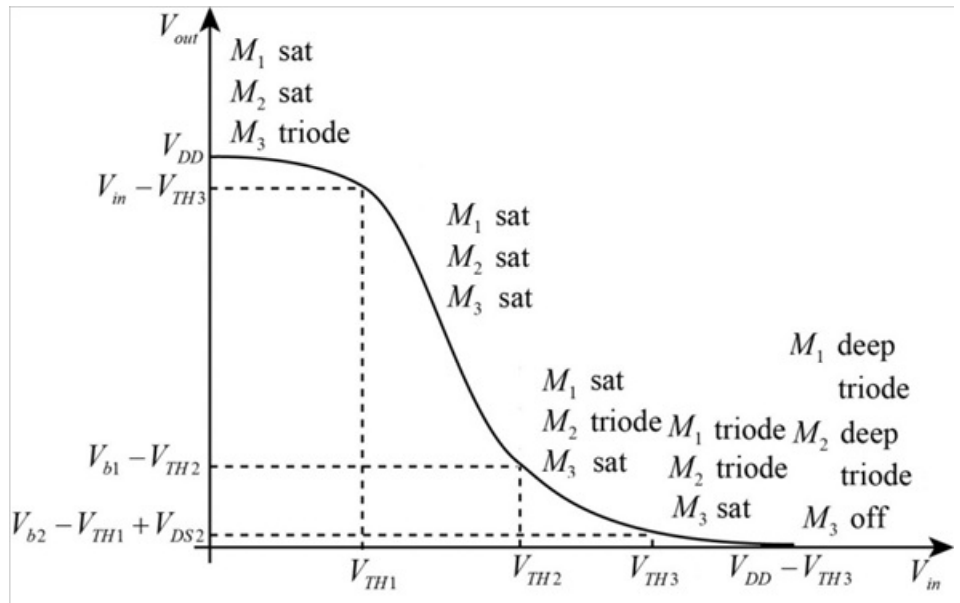
\includegraphics[width=1\linewidth]{3.17-3}
	\end{minipage}
	\caption*{图3} %最终文档中希望显示的图片标题
\end{figure}

\scalebox{3}{(d)}



由图3当$V_{in}<V_{TH2}$时

$I_{D1}=I_{D2}$

$\frac{1}{2}\mu_nC_{ox}\frac{W}{L}(V_{b2}-V_{TH1})^2=\frac{1}{2}\mu_nC_{ox}\frac{W}{L}(V_{b1}-V_{out}-V_{TH2})^2$

\begin{figure}[H] %H为当前位置,!htb为忽略美学标准,htbp为浮动图形
	\begin{minipage}{\linewidth}
		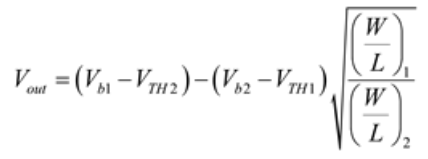
\includegraphics{3.17-4}
	\end{minipage}
\end{figure}














		\begin{figure}[H] %H为当前位置,!htb为忽略美学标准,htbp为浮动图形
	\begin{minipage}{\linewidth}
		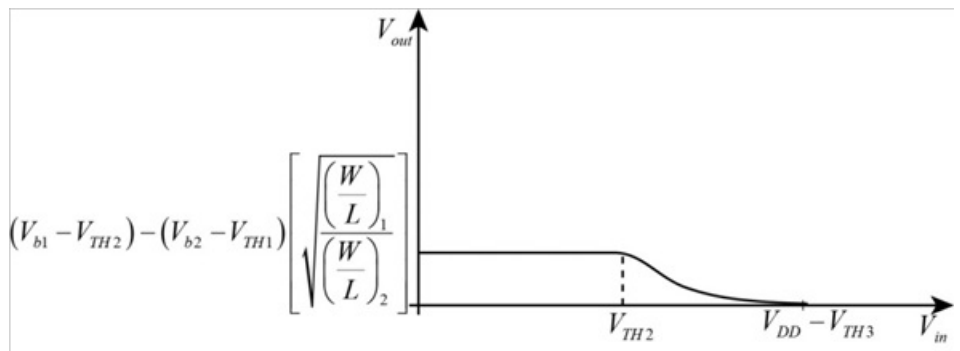
\includegraphics[width=1\linewidth]{3.17-5}
	\end{minipage}
	\caption*{图4} %最终文档中希望显示的图片标题
\end{figure}

\color{green}{
	
	\{
	
	(a)横轴的$V_{TH2}=V_{b}-V_{TH2}+V_{GS1}$?
	
	(c)$M_3$同时关和线性区?
	
	\}
	
}

\color{black}{}